\section{\icecube{}}
The \icecubeneutrinoobservatory{} is located close to the geographic South Pole
  in proximity to the Amundsen-Scott South Pole Station.
% █ Why the South Pole?
It utilizes the optically clear Antarctic ice as detector material,
  with a total detector volume of \SI{1}{\cubic\kilo\meter} \cite{icecube_aartsen}.
The detector is composed of \num{86} strings,
  each consisting of \num{60} \acp{DOM},
    which are positioned
      \SI{17}{\meter} apart along the string
      at depths ranging from \SI{1450}{\meter} to \SI{2450}{\meter} below the surface \cite{icecube_aartsen}.
Each of the \num{5160} \acp{DOM} is equipped with a sensitive \ac{PMT},
  which detects the Cherenkov light emitted by charged particles
    that interact with the ice.
%
\autoref{fig:img:icecube} shows a schematic of the \icecube{} detector.

% \icecube{} detects 275 atmospheric neutrinos daily and about 100,000 per year.


\begin{figure}
  \centering
  % COULDDO: I made this pretty small to accommodate for newly added text.
  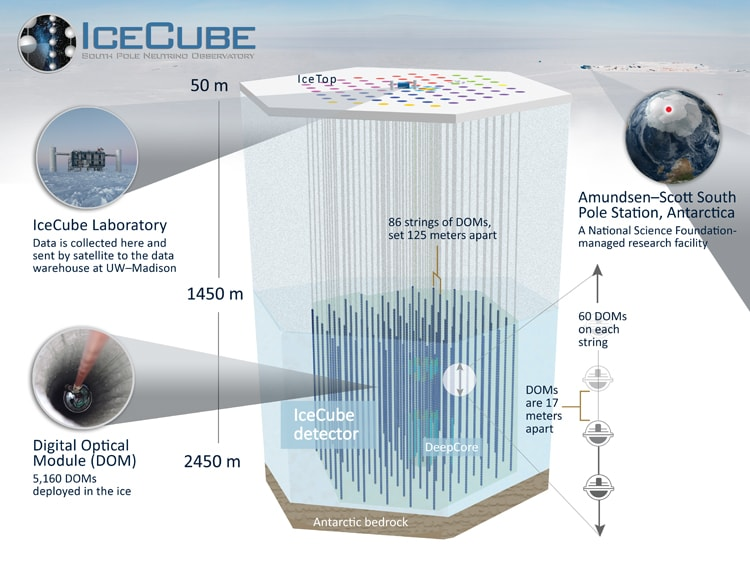
\includegraphics[width=0.65\textwidth]{content/img/icecube_detector_schematic.jpg}
  \caption{
    % Schematic representation
    % Overview
    Infographic
    of the \icecubeneutrinoobservatory{} \cite{icecube_homepage}.
    Each dot represents a \ac{DOM}.
    % COULDDO: longer description
  }
  \label{fig:img:icecube}
\end{figure}


% \subsection{Detection Principle}

% █ Interaction with matter
Neutrinos interact with matter via the weak interaction.
In order to compensate for the low cross-section of the weak interaction,
  the effective detector volume is maximized by utilizing existing naturally occurring detector materials,
  such as
    the Earth's atmosphere,
    the sea,
    or the ice in the Antarctica.
%
When a neutrino interacts with a nucleus in the ice,
it produces a charged lepton and a neutrino.
The charged lepton then produces a Cherenkov light cone
as it propagates through the ice
with greater speed than the speed of light in the ice.
% COULDDO: add Cherenkov figure (in appendix)
The light is detected by the \acp{PMT}
  and
    % (in the case of muon neutrinos, mostly)
  the direction of the neutrino can be reconstructed
    from the position of the \acp{DOM}
      that detected the light.
The intensity of the light and the number of \acp{PMT} that detected it
  are used to determine the energy of the neutrino.
%
\icecube{}
  % (without \emph{DeepCore} and \emph{IceTop})
is sensitive to
  the approximate neutrino energy range
    from \si{\giga\electronvolt} to \si{\peta\electronvolt} \cite{icecube_aartsen}
    % NOTE: “100 GeV for most IceCube analyses” (→ icecube_aartsen)
    % from \SI{E7}{\electronvolt} to \SI{E21}{\electronvolt}. % source: Wikipedia / https://web.archive.org/web/20060909003706/http://icecube.wisc.edu/pub_and_doc/reviews_and_meetings/June2002_NRC-Review/presentations/nrc_halzen.pdf
  and therefore primarily to atmospheric and \ac{AGN} neutrinos.
Higher energies require even larger detector volumes.

Depending on the flavor of the leptons,
different types of interactions occur,
allowing to determine the flavor of the neutrino in turn.
%
% NOTE: The following differentiation is a little hand-wavy.
% For example, ALL neutrino flavors can shower to produce spherical signatures (→ icecube_aartsen).
%
% ▒ µ-neutrinos
% NOTE: The Monte Carlo data used in this work only contains muon neutrinos.
% ORIG[icecube_aartsen]: Track-like events originate from a charged-current interaction of a high-energy muon neutrino with a nucleus, producing a hadronic shower at the vertex and an outgoing muon that emits Cherenkov light in a cone along its track. The angular resolution for muon tracks and hence the incident neutrino direction is typically 0.6°, confirmed by analysis of the shadows of the Moon and Sun in cosmic rays [19, 20]. Muons with energies above a critical energy, about 1 TeV in ice, predominantly lose energy by radiative processes that exhibit a stochastic behavior with large fluctuations. This results in large variability in the amount of energy deposited for different muons of the same energy.
%
Muon neutrinos are detected as \emph{tracks} \cite{icecube_aartsen}
  which originate from a charged-current interaction of a high-energy muon neutrino with a nucleus.
They have a good angular resolution
  because muons typically fall under the Cherenkov limit as soon as they scatter.
%
% ▒ e-neutrinos
% ORIG[Wikipedia]: IceCube is more sensitive to muons than other charged leptons, because they are the most penetrating and thus have the longest tracks in the detector. Thus, of the neutrino flavors, IceCube is most sensitive to muon neutrinos. An electron resulting from an electron neutrino event typically scatters several times before losing enough energy to fall below the Cherenkov threshold; this means that electron neutrino events cannot typically be used to point back to sources, but they are more likely to be fully contained in the detector, and thus they can be useful for energy studies. These events are more spherical, or "cascade"-like, than "track"-like; muon neutrino events are more track-like.
%
Electron neutrinos,
  on the other hand,
are detected as \emph{cascades} \cite{icecube_aartsen}.
Contrary to muons,
  electrons typically scatter several times before falling below the Cherenkov threshold,
    therefore prohibiting the reconstruction of the neutrino direction.
On the other hand,
  they are more likely to be fully contained in the detector,
    which makes them useful for energy studies \cite{icecube_aartsen}.
%
% ▒ τ-neutrinos
% ORIG[Wikipedia]: Tau leptons can also create cascade events; but are short-lived and cannot travel very far before decaying, and are thus usually indistinguishable from electron cascades. A tau could be distinguished from an electron with a "double bang" event, where a cascade is seen both at the tau creation and decay. This is only possible with very high energy taus. Hypothetically, to resolve a tau track, the tau would need to travel at least from one DOM to an adjacent DOM (17 m) before decaying. As the average lifetime of a tau is 2.9×10−13 s, a tau traveling at near the speed of light would require 20 TeV of energy for every meter traveled.[17] Realistically, an experimenter would need more space than just one DOM to the next to distinguish two cascades, so double bang searches are centered at PeV scale energies. Such searches are underway but have not so far isolated a double bang event from background events.[citation needed]
%
A third type of signature is the
    \emph{double bang} \cite{kowalski2017}
    or \emph{lollipop} \cite{neutrinos_beacom},
  which very high energy tau neutrinos could produce.
It has not been observed so far \cite{neutrinos_aartsen_tau}.
%
Examples of interactions and corresponding detector patterns are shown in \autoref{fig:img:icecube:interactions}.

\phantomsection \label{sec:neutrino_astronomy:icecube:up_going}
Not only neutrinos can leave traces in the detector, % interact with the ice,
  but also atmospheric muons.
For this reason,
  the detection is mostly limited to \emph{up-going} events \cite{icecube_aartsen},
  % ($\SI{0}{\degree} < \theta < \SI{180}{\degree}$)
  % ORIG: Up-going events for all triggered energies are selected, while only high-energy down-going tracks are selected to avoid the large background of down-going atmospheric muons at lower energies.
    because muons
      – in contrast to neutrinos –
    are mostly blocked by the Earth's mass.


% COULDDO: If there were more space, one could write about:
% - Triggering / reconstruction / feature extraction
% - Numbers and facts
% - Achievements
